\documentclass{beamer}

% german content
\usepackage[ngerman]{babel}

% bibliography
\usepackage[
backend=biber,
style=authoryear,
citestyle=authoryear,
autocite=footnote
]{biblatex}
\addbibresource{bibliography.bib}

% images
\usepackage{graphicx}
\graphicspath{ {images/} }

\title{Import/Export von saisonalen Produkten}
% \subtitle{}
\author[Dao, Gabele, Neidel, Neuthor, Spannbauer, Wiegandt]{
  Dao, Duc Trung \and\\
  Gabele, Jörg \and\\
  Neidel, Jonathan \and\\
  Neuthor, Marco \and\\
  Spannbauer, Daniel \and\\
  Wiegandt, Lisa-Marlen
}
\date{Januar 2020}
\institute{HTW Berlin, Angewandte Informatik}
\logo{
\includegraphics[width=1cm]{logo.png}}

% theme + color theme
\usetheme{Szeged}
\usecolortheme{whale}
% see: https://deic-web.uab.cat/~iblanes/beamer_gallery/index.html

\begin{document}
\frame{\titlepage}

\begin{frame}
\frametitle{Abstract}
Abstract here
\end{frame}

% show all section names
\begin{frame}
\frametitle{Table of Contents}
\tableofcontents
\end{frame}
% how to exclude a section from toc: https://tex.stackexchange.com/a/66633


\section{Warennummern}
\begin{frame}
\frametitle{Warenverzeichnis}
Das \textbf{Warenverzeichnis für die Außenhandelsstatistik} (WA) führt die
achtstelligen Statistischen Warennummern auf, mit deren Hilfe Waren
eindeutig gekennzeichnet werden können.
\end{frame}

\begin{frame}
\frametitle{Warenverzeichnis}
\begin{figure}[h]
    \centering
    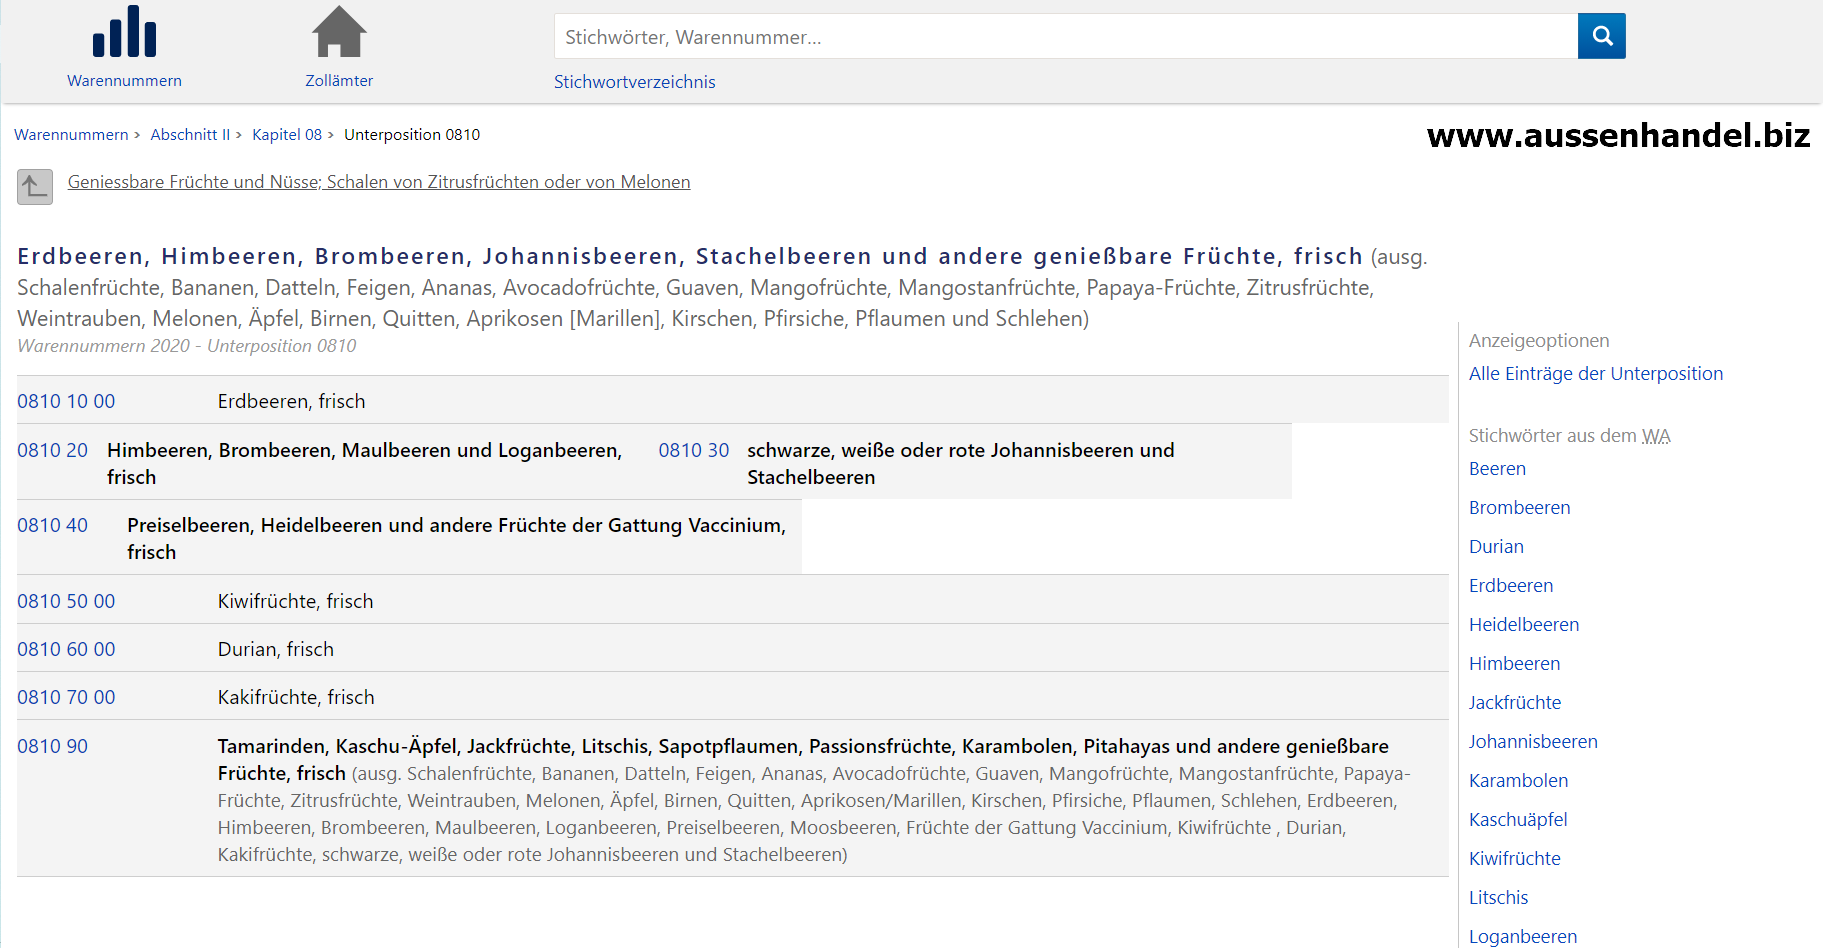
\includegraphics[height=5.5cm]{warennummern}
    \caption{https://aussenhandel.biz}
  \end{figure}
\end{frame}

\begin{frame}
\frametitle{Aufbau WA}
EU-eineitliche Kennzeichnungssystematik
\end{frame}

\begin{frame}
\frametitle{WA: Lebensmittel}
  \begin{figure}[h]
    \centering
    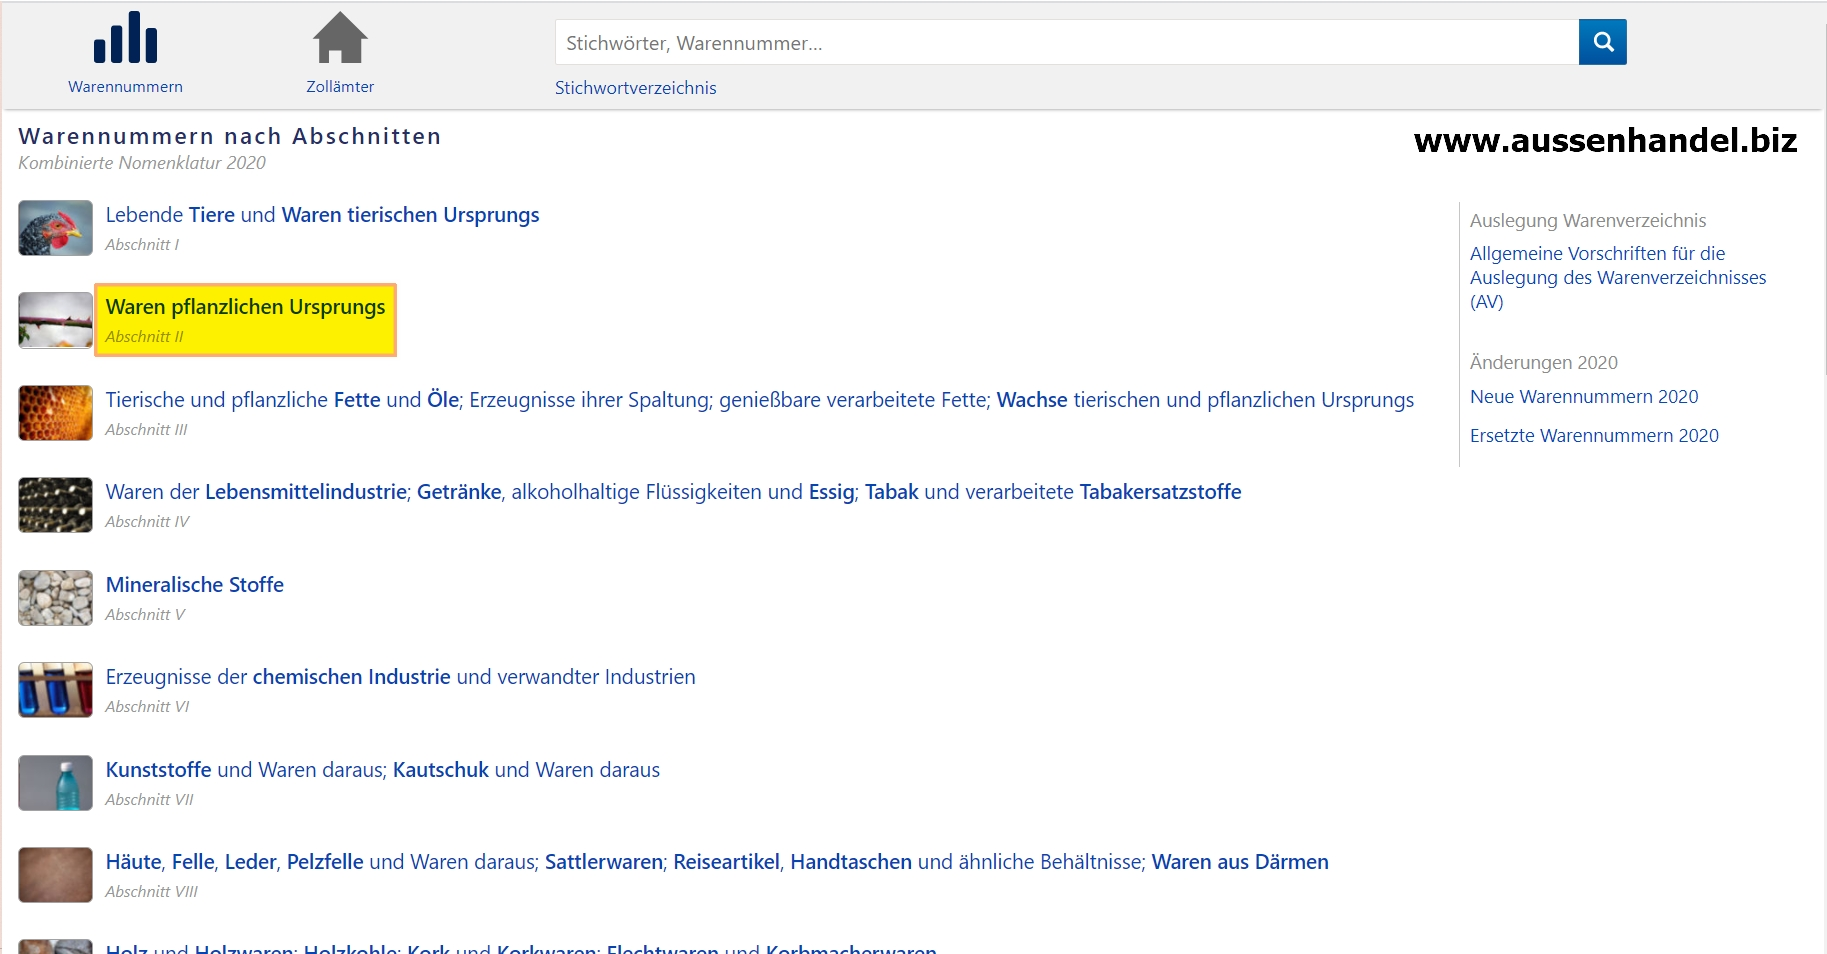
\includegraphics[height=5.5cm]{wa}
    \caption{https://aussenhandel.biz}
  \end{figure}
\end{frame}

\begin{frame}
\frametitle{Beispiel: Spargel}
  \begin{figure}[h]
    \centering
    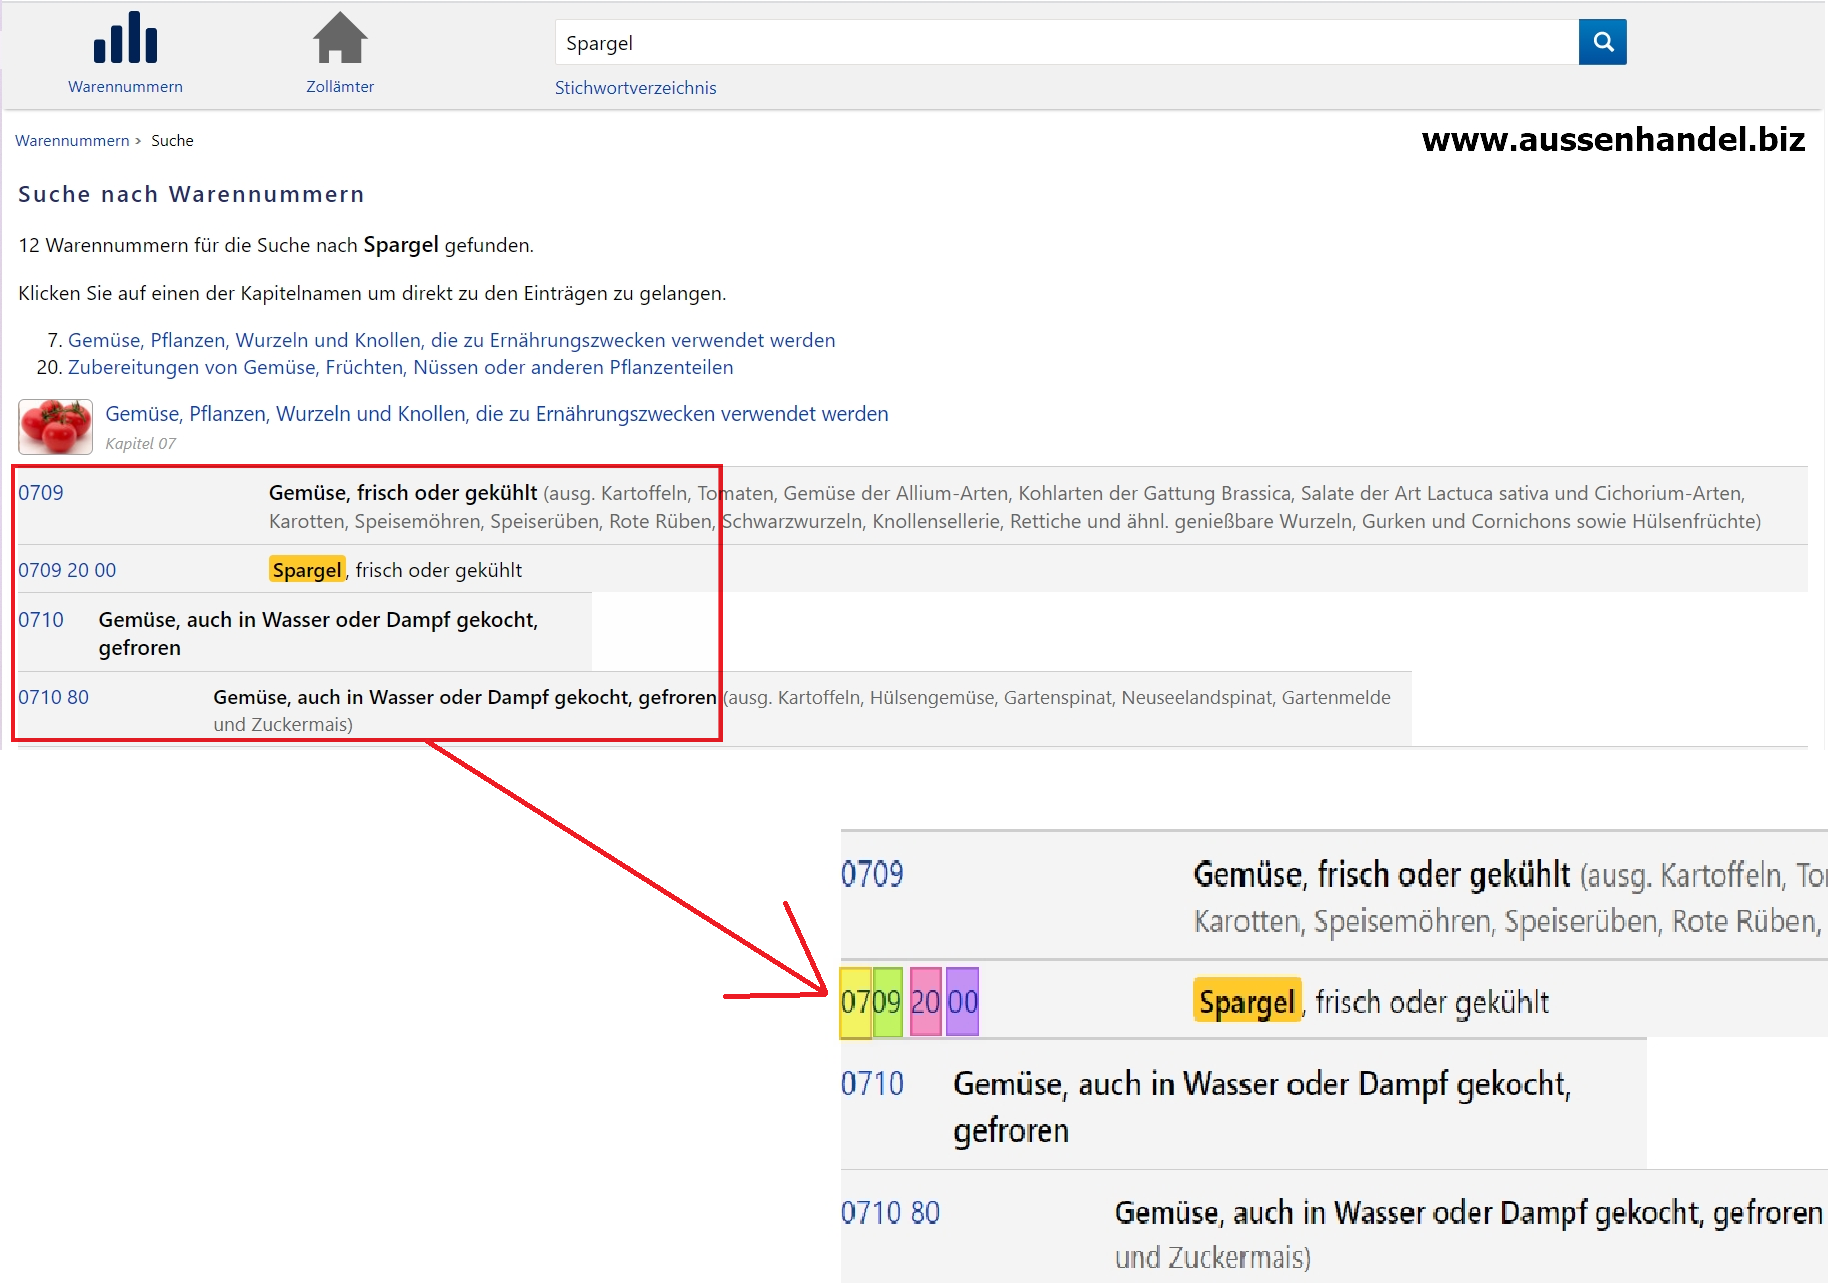
\includegraphics[height=6cm]{wa-spargel}
    \caption{https://aussenhandel.biz}
  \end{figure}
\end{frame}

\begin{frame}
\frametitle{Beispiel: Spargel}
      \begin{itemize}
        \item
07: Kapitel 7 von Abschnitt II
        \item
09: Nummer von Gemüse, frisch oder gekühlt
        \item
20: Nummer von Ware Spargel
        \item
00: Kategorie von Ware Spargel.
      \end{itemize}
\end{frame}

% \begin{frame}
% \frametitle{<++>}
% <++>
% \end{frame}

% bibliography
% \break
% \printbibliography

\end{document}
